\section{Evaluation}
\begin{table}
  \begin{scriptsize}
  \begin{tabular}{p{0.3\columnwidth}p{0.7\columnwidth}}
  SKETCH construct & Description \\
  \hline
  MuxN(a1, a2, \dots, aN) & \pbox{0.7\columnwidth}{N-to-1 multiplexer with enable bit.\\If enabled, return one of a1, a2, \dots aN.\\If disabled, return 0.}\\
  Opt(a)        & Return a or 0. \\
  rel\_op(x, y) & Return one of $x < y$, $x > y$, $x != y$, $x == y$.\\
  C() & Return an integer constant in the range [0, 31].\footnote{We restrict constants to 5 bits because all constants in our dataplane algorithms are under 32. Larger ranges increase synthesis time.} \\
  x, y & State variables \\
  pkt\_1, pkt\_2 & Packet fields \\
  \end{tabular}
  \end{scriptsize}
  \caption{SKETCH shorthand used in atom templates}
  \label{tab:sketch_constructs}
\end{table}

%TODO: Add compilation times
%TODO: Add number of stages for each algorithm.
%TODO: Mention something about how propagation delay goes up as complexity increases.
%TODO: Is there a good technical reason why every \absmachine machine
% should have exactly one large stateful atom as opposed to many small stateful atoms?
\label{s:eval}
\begin{table*}[!t]
  \begin{scriptsize}
  \begin{tabular}{|p{0.15\textwidth}|p{0.8\textwidth}|}
  \hline
  Atom template & SKETCH shorthand\\
  \hline
  Write &
  {\begin{lstlisting}[style=customctable]
  x = mux2(pkt.f, ??);
  \end{lstlisting}} \\
  \hline
  ReadAddWrite (RAW) &
  {\begin{lstlisting}[style=customctable]
  x = mux2(x, ??) + mux2(??, pkt.f);
  \end{lstlisting}} \\
  \hline
  \pbox{0.15\textwidth}
  {Predicated\\
  ReadAddWrite (PRAW)} &
  {\begin{lstlisting}[style=customctable]
  if(mux2(x, ??) rel_op mux3(pkt.f1, pkt.f2, ??)) {
    x = mux2(x, ??) + mux3(??, pkt.f1, pkt.f2);
  }
  \end{lstlisting}} \\
  \hline
  \pbox{0.15\textwidth}
  {If-Else\\
   ReadAddWrite\\
   (If-Else RAW)} &
  {\begin{lstlisting}[style=customctable]
  if(mux2(x, ??) rel_op mux3(pkt.f1, pkt.f2, ??)) {
    x = mux2(x, ??) + mux3(??, pkt.f1, pkt.f2);
  } else {
    x = mux2(x, ??) + mux3(??, pkt.f1, pkt.f2);
  }
  \end{lstlisting}} \\
  \hline
  \pbox{0.15\textwidth}
  {4-operand instructions\\
   (4oper)} &
  {\begin{lstlisting}[style=customctable]
  if(mux2(x, ??) rel_op mux3(pkt.f1, pkt.f2, ??)) {
    x = mux2(x, ??) + mux3(??, pkt.f1, pkt.f2) - mux3(??, pkt.f1, pkt.f2);
  } else { 
    x = mux2(x, ??) + mux3(??, pkt.f1, pkt.f2) - mux3(??, pkt.f1, pkt.f2);
  }
  \end{lstlisting}} \\
  \hline
  Paired Updates (Pairs) &
  {\begin{lstlisting}[style=customctable]
  bit pred1 = mux3(x, y,  ??) rel_op mux3(pkt.f1, pkt.f2, ??);
  bit pred2 = mux3(x, y,  ??) rel_op mux3(pkt.f1, pkt.f2, ??);
  if (pred1) {
    x = mux2(x, ??) + mux3(??, pkt.f1, pkt.f2) - mux3(??, pkt.f1, pkt.f2);
    y = mux2(x, ??) + mux3(??, pkt.f1, pkt.f2) - mux3(??, pkt.f1, pkt.f2);
  } else if (pred2) {
    x = mux2(x, ??) + mux3(??, pkt.f1, pkt.f2) - mux3(??, pkt.f1, pkt.f2);
    y = mux2(x, ??) + mux3(??, pkt.f1, pkt.f2) - mux3(??, pkt.f1, pkt.f2);
  }
  \end{lstlisting}} \\
  \hline
  \end{tabular}
\end{scriptsize}
  \caption{Atom templates used in evaluation. rel\_op $\in \{<, >, != , ==\}$ stands for a relational operator. ?? refers to a SKETCH hole that can be filled in with an unsigned integer in the range $[0, 2^n]$.}
  \label{tab:templates}
\end{table*}

\begin{table*}[!t]
\begin{tabular}{|p{0.20\textwidth}|p{0.74\textwidth}|}
\hline
Algorithm & Stateful computation \\
\hline
Bloom filter & \pbox{0.74\textwidth}{Set membership bit on every packet.}\\
\hline
Heavy Hitters~\cite{opensketch} & Increment Count-Min Sketch~\cite{cormode} on every packet. \\
\hline
Flowlets~\cite{flowlets} & Update saved next hop if flowlet threshold is exceeded. \\
\hline
RCP~\cite{rcp} & Accumulate RTT sum if RTT is under maximum allowable RTT. \\
\hline
Sampling & \pbox{0.74\textwidth}{Sample/Mark a packet if packet count reaches N; reset count at N.} \\
\hline
HULL~\cite{hull} & Update counter for virtual queue.\\
\hline
CONGA~\cite{conga} & \pbox{0.74\textwidth}{Update best path's utilization/id if we see a better path.\\
                                           Update best path utilization alone if it changes.} \\
\hline
trTCM~\cite{trTCM} & \\
\hline
CoDel~\cite{codel} & \\
\hline
\end{tabular}
\caption{Data-plane algorithms}
\label{tab:algos}
\end{table*}

\begin{figure*}[!t]
  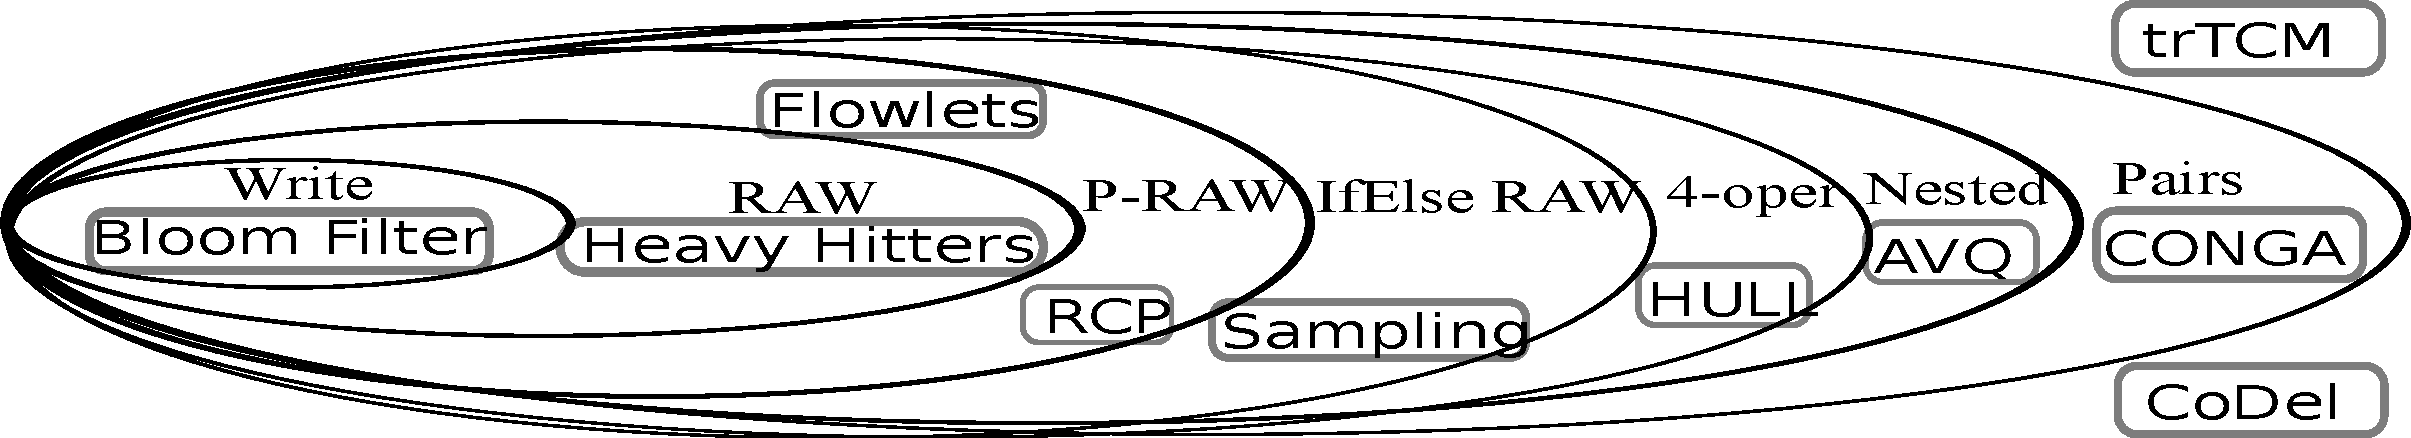
\includegraphics[width=\textwidth]{atom_hierarchy.pdf}
  \caption{Containment hierarchy of \absmachine machines and what data-plane algorithms each can implement.}
\label{fig:eval}
\end{figure*}

%10. Alvin's feedback: Write about our experience writing these programs. Similar to Steven Chong's PLDI paper.
To evaluate \pktlanguage, we express several well-known data-plane algorithms
(Table~\ref{tab:algos}) using \pktlanguage and determine if they are
implementable on different \absmachine machines that provide different stateful
atoms (Table~\ref{tab:templates}).

\subsection{Experimental procedure}
As mentioned before, we consider only stateful atoms by assuming stateless
codelets map one-to-one to stateless atoms for all \absmachine machines. For
simplicity, the stateful atoms only permit updates to state variables and
forbid packet field updates resulting from these state updates.  Assuming the
\absmachine machine provides an atom to read a state variable\footnote{The
inability to read a state variable renders it powerless!}, such packet updates
can be treated as stateless operations in subsequent pipeline stages. We
represent atoms using their atom templates in Table~\ref{tab:templates},
employing a shorthand notation for SKETCH (Table~\ref{tab:sketch_functions}).

%Anirudh->Alvin: Is it clear now that each machine provides exactly one atom.
We also assume every \absmachine machine provides exactly one stateful atom.
Table~\ref{tab:templates} gradually increases the capability of this single
atom provided by a \absmachine machine.  The atoms in Table~\ref{tab:templates}
, and the \absmachine machines providing them, form a containment hierarchy
(Figure~\ref{fig:eval}): each atom is strictly more expressive than its
predecessor and hence can express all data-plane algorithms that its
predecessor can.

We now consider every atom/\absmachine machine from Table~\ref{tab:templates},
and every data-plane algorithm from Table~\ref{tab:algos} to determine if each
algorithm is \textit{implementable} on a particular \absmachine machine. We
say an algorithm is implementable on a \absmachine machine, if every stateful
codelet within the data-plane algorithm can be mapped (\S\ref{ss:code_gen}) to
the single stateful atom provided by the \absmachine machine.

\subsection{Interpreting these results}
Figure~\ref{fig:eval} tells a network programmer if a particular data-plane
algorithm can be implemented at line rate, assuming the \absmachine machine
provides a particular stateful atom. For an ASIC engineer designing
programmable switching chips, the same figure describes the algorithms that are
implementable on a particular \absmachine machine. For instance, a \absmachine
machine with the paired updates atom can implement all six algorithms shown in
Figure~\ref{fig:eval}, while a machine with a simpler increment atom can
implement only two.

These results will change as programmable switches evolve and network
programmers push chip boundaries with new algorithms.  The larger takeaway is
that programming in \pktlanguage allows us to rigorously determine if a
particular high-level algorithm is implementable at line rate on a particular
\absmachine machine. Conversely, it tells us if a particular \absmachine
machine suffices to implement a large number of algorithms.
